% !TEX root = ReviewDraft.tex



\section{The entanglement wedge and the black hole interior} \label{wedge}


 
 The central dogma talks about some degrees of freedom which suffice to describe the black hole from the outside. A natural question to ask is whether these degrees of freedom also describe the interior.   We have several possibilities: 
 
 a) They do not describe the interior. 
 
 b) They describe a portion of the interior. 
 
 c) They describe all of the interior. 
 
A guiding principle has been the formula for the fine-grained entropy of the black hole. This formula is supposed to give us the entropy of the density matrix that describes the black hole from the outside, if we are allowed to make arbitrarily complicated measurements. 
 We have seen that the answer for the entropy depends on the geometry of the interior. However, it only depends on the geometry and the state of the quantum fields up to the extremal   surface. Note that if we add an extra spin in an unknown state between the cutoff surface and the extremal  surface, then it will modify the fine-grained entropy. 
 
 Therefore it is natural to imagine that the degrees of freedom in the central dogma describe the geometry up to the minimal surface. If we know the state on any spatial region, we also know it in the causal diamond associated to that region, recall figure \ref{Diamond}. This has historically been called the ``entanglement wedge" \cite{Czech:2012bh,Wall:2012uf,Headrick:2014cta}. Following our presentation perhaps a better name would be ``the fine-grained entropy region," but we will not attempt to change the name. 

As a first example, let us look again at a black hole formed from collapse but before the Page time. The minimal surface is now a vanishing surface at the origin and the entanglement wedge of the black hole is the region depicted in green in figure  \ref{EWfig}a.   

\begin{figure}[ht]
\begin{center}
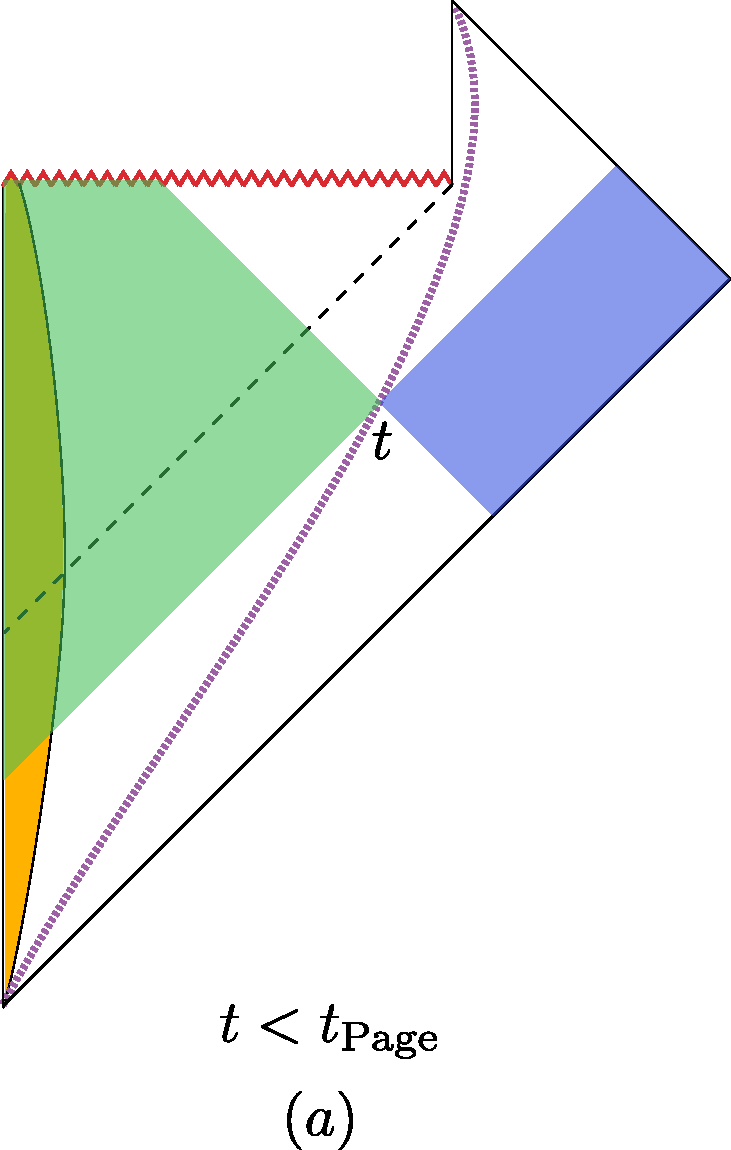
\includegraphics[scale=.35]{figures/EWa.pdf} \ \ \ \ \ \  \ \
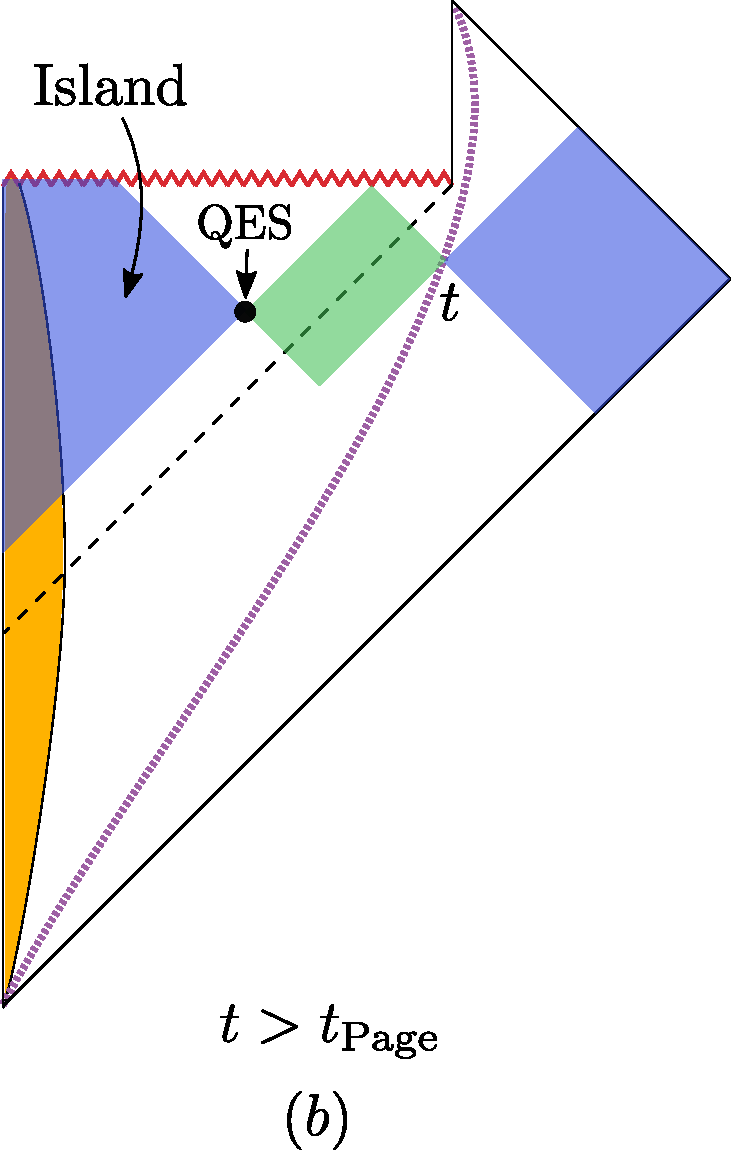
\includegraphics[scale=.35]{figures/EWb.pdf}  \ \ \ \ \ \  \ \
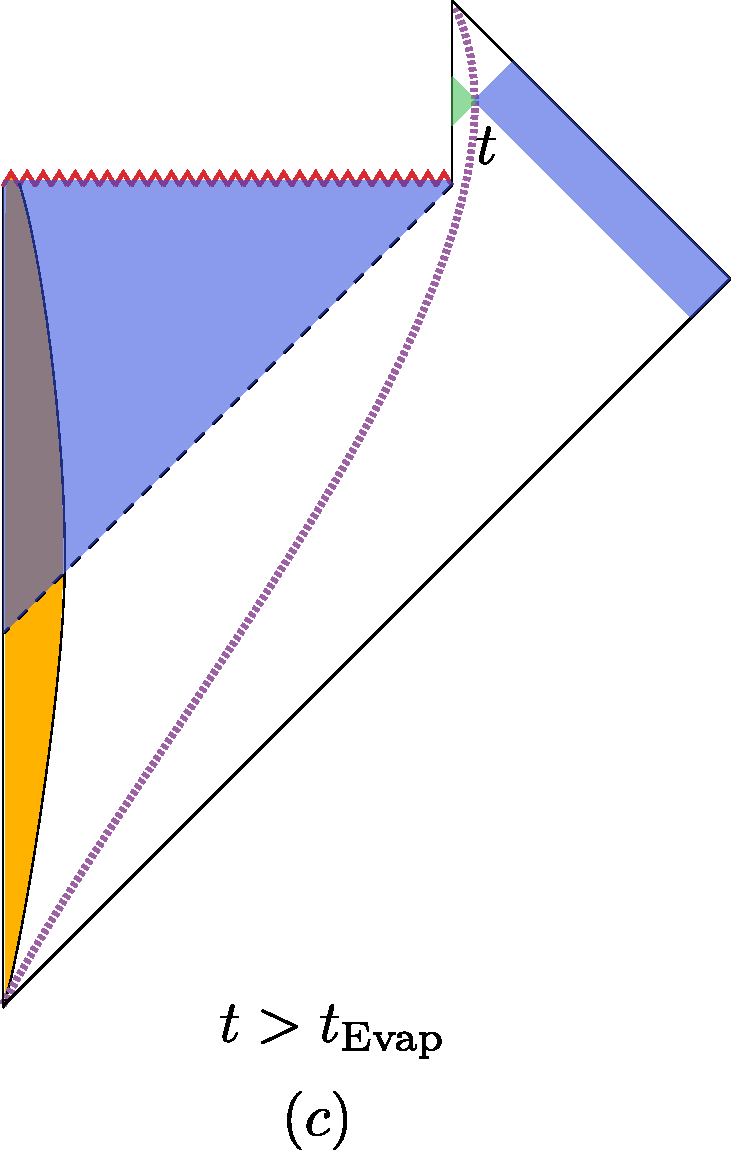
\includegraphics[scale=.35]{figures/EWc.pdf} 
\caption{ In green we show the entanglement wedges of the black hole and in blue the entanglement wedges of the radiation region. Different figures show the wedges at different times. They are different because there is transfer of quantum information through the cutoff surface. To describe the white regions we need information both from the black hole region and the radiation region.   }
\label{EWfig}
\end{center}
\end{figure}


As a second   example, we can look at the entanglement wedges of both the black hole and the radiation at late times, larger than the Page time. These are shown in figure \ref{EWfig}(b). 
The idea is that the black hole degrees of freedom describe the region of the spacetime in the black hole entanglement wedge while the radiation describes the degrees of freedom in the radiation entanglement wedge. It is important that the degrees of freedom that describe the black hole only describe a portion of the interior, the green region in figure \ref{EWfig}(b). The rest of the interior is encoded in the radiation. 

 
Note how this conclusion, namely that the interior belongs to the entanglement wedge of the radiation, follows from the same guiding principle of using the fine-grained entropy. Since the fine-grained entropy of the radiation after the Page time contains the interior as part of the island, its entropy is sensitive to the quantum state of that region; a spin in a mixed state in the island contributes to the fine-grained entropy of the radiation.


Finally, as a third example,  we can consider a fully evaporated black hole, see figure \ref{EWfig}(c). In this case the region inside the cutoff surface is just flat space. The entanglement wedge of the radiation includes the whole black hole interior. This picture assumes that nothing too drastic happens at the endpoint of the evaporation. 

    
 
 So far we have been a bit vague by the statement that we can ``describe'' what is in the entanglement wedge. A more precise statement is the ``entanglement wedge reconstruction hypothesis," which says that if we have a relatively small number of qubits  in an unknown state but located inside the entanglement wedge of the black hole, then by performing   operations on the black hole degrees of freedom, we can read off the state of those qubits. 
   This  hypothesis is supported by general principles of quantum information. Let us consider the case when the radiation entanglement wedge covers most of the interior, as in figure \ref{EWfig}(b).  Then the action of the  black hole  interior  operators of the semiclassical description   affect the entropy of radiation, according to the gravitational entropy formula. Assuming that this formula captures  the true entropy of the exact state of radiation, this means that these operators are changing this exact state \cite{Jafferis:2015del,Dong:2016eik}, see also \cite{Almheiri:2014lwa}.   Then it follows from general quantum information ideas that there is a map, called the 
   Petz map \cite{PetzBook},  that allows us to recover the information \cite{Cotler:2017erl}. In the context of simple gravity theories, this map can be constructed using the gravitational path integral \cite{Penington:2019kki}, again via the replica method. This provides a formal argument, purely from the gravitational side, for the validity of the hypothesis. 
    The actual quantum operations we would need to perform on the radiation are expected to be exceedingly complex, with a complexity that is (roughly) exponential in the black hole entropy 
    \cite{Brown:2019rox,Kim:2020cds}.
  
 For black holes after the Page time,  most of the interior is {\it not} described by the black hole degrees of freedom appearing in the central dogma. In fact, it is described by the radiation degrees of freedom. At late times, these are much more numerous than the area of the horizon. 
	
	 
	Note that there is an unfortunate language problem which sometimes gets in the way of the concepts we are trying to convey. The reason is that there are two {\it different} things that people might want to call ``black hole degrees of freedom." We have been calling ``black hole degrees of freedom'' the ones that appear in the central dogma. They are the ones that are sufficient to describe the black hole from the outside. These are not very manifest in the gravity description. The other possible meaning would refer to the quantum fields living in the semiclassical description of the black hole interior. As we explained above, depending on which side of the quantum extremal surface they lie on, these degrees of freedom can be encoded  either  in the Hilbert space  appearing in the central dogma or the Hilbert space living in the radiation region.   	
	
	 
	  This observation also solves an old puzzle with the interpretation of the  Bekenstein-Hawking   area formula that was raised by Wheeler \cite{WheelerBag}. 
 He pointed out that there exist classical geometries which look like a black hole from the outside but that inside can have arbitrarily large entropy, larger than the area of the horizon. He named them ``bags of gold," see figure \ref{BagGold}. The solution to this puzzle is the same. When the entropy in the interior is larger than the area of the neck  the entanglement wedge of the black hole degrees of freedom will only cover a portion of the interior, which does not include that large amount of entropy \cite{WallGold}.   In fact, the geometry of an evaporating black hole after the Page time is a bit like that of the ``bag of gold'' examples. 
 
 \begin{figure}[ht]
\begin{center}
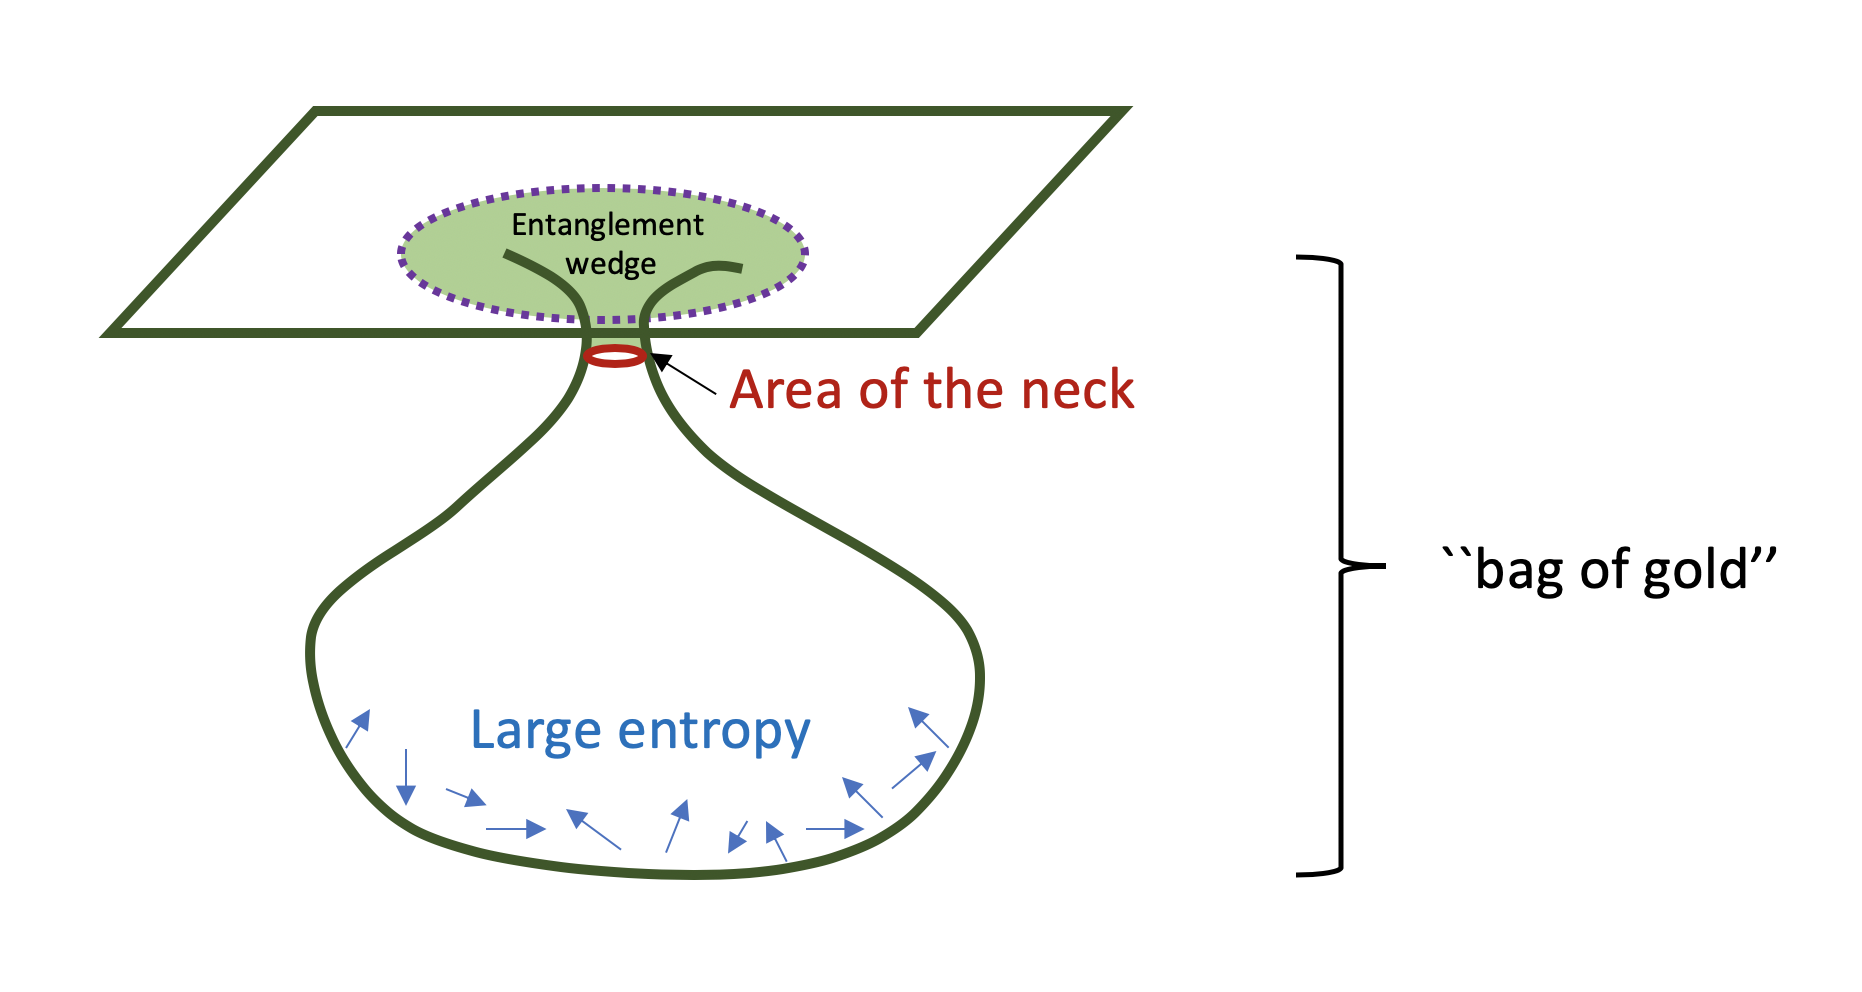
\includegraphics[scale=.35]{figures/BagGold}  
\caption{  Wheeler's ``bag of gold'' geometry. It is a spatial geometry that is asymptotically flat and has a narrow neck with a big ``bag'' containing some matter. It obeys the initial value constraints of general relativity. From the point of view of the outside the geometry evolves into a black hole whose area is given by the area of the neck. The entropy inside the bag can be much larger than the area of the neck. Under these circumstances the fine-grained entropy of the exterior is  just   given by the  area of the neck and the entanglement wedge does  not include the interior.  }
\label{BagGold}
\end{center}
\end{figure}

